% CUSTOM TEMPLATE FOR SOLUTIONS STARTS
\documentclass[answers]{exam}
 
 \usepackage{graphicx}
 \usepackage{float}
 \usepackage{amsmath}
 \usepackage{amsfonts}
 \usepackage{framed}
 \usepackage{algorithmicx}
 \usepackage{algpseudocode}
 \newcommand{\ans}[1]{\begin{framed}{\textbf{Answer:} #1}\end{framed}}
 \newcommand{\sol}{\uplevel{\textsc{Solution:}}}
 \newenvironment{answer}{%
     \renewcommand{\solutiontitle}{\noindent\textbf{Answer:}\enspace}
     \begin{solution}
     }{%
     \end{solution}
     \renewcommand{\solutiontitle}{\noindent\textbf{Solution:}\enspace}
 }
% CUSTOM TEMPLATE FOR SOLUTIONS ENDS

% First we setup the header and footer
\pagestyle{headandfoot}
\runningheadrule
\runningfootrule
\header{COL351: Analysis and Design of Algorithms (CSE, IITD, Semester-I-2020-21)}{}{Quiz 5}
\footer{}{\thepage  \, of \numpages}{}
 
% We want the points for each question displayed on the left
%\pointname{points}
%\pointsinmargin
 
% Automatically total the points - make sure to compile TWICE
\addpoints
 
\begin{document}


\vspace{0.1in}


\vspace{0.1in}
% Some general text together with number of questions and total points possible
There are \numquestions\, questions for a total of \numpoints\, points.
\vspace{0.1in}
\hrule
 \vspace{0.2in}
\begin{questions}
 
\question[3] 

Consider the flow network below and the mapping $f$ from edges to numbers:

    \begin{center}
        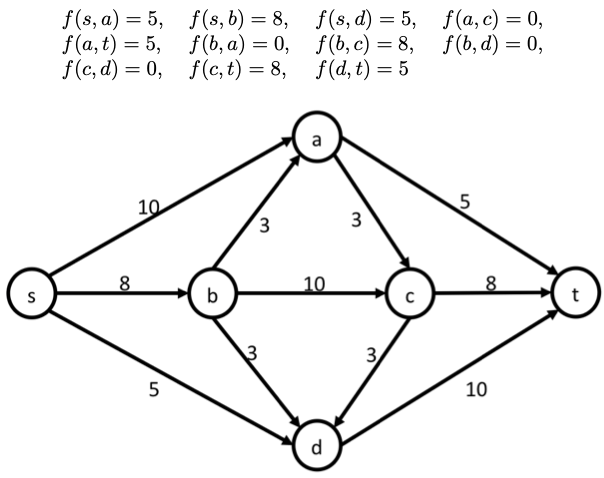
\includegraphics[scale=0.9]{img/flow1.png}
    \end{center}

    \begin{parts}

        \part
        $f$ is an $s$-$t$ flow.
        \begin{answer}
            True
        \end{answer}
        \part
        $f$ is an $s$-$t$ flow with maximum value.
        \begin{answer}
            False
        \end{answer}
        \part Give an $s$-$t$ cut $(A, B)$ with minimum capacity. You can specify a minimum cut by giving sets $A$ and $B$.
        \begin{answer}
            $A = \{s, a\}, B = \{b, c, d, t\}$
        \end{answer}
        \part What is the capacity of minimum-cut?
        \begin{answer}
            21
        \end{answer}

    \end{parts}

\question[7]

There is an $n \times n$ grid in which some cells are empty and some are filled. The empty/filled cells are given by an $n \times n$, 0/1 matrix $F$. Cell $(i, j)$ is empty iff $F[i, j] = 0$. You have
    unbounded supply of $2 \times 1$ tiles (called dominoes). Each domino could be placed on the empty cells of the grid in horizontal and vertical manner (note that you need two consecutive empty
    cells on the grid for doing this). The problem is to determine if the grid can be covered by placing these $2 \times 1$ dominos such that each empty cell is covered by exactly one domino.

(The figure below shows an example of a $4 \times 4$ grid that can be covered using $2 \times 1$ domino tiles.)

\begin{center}
    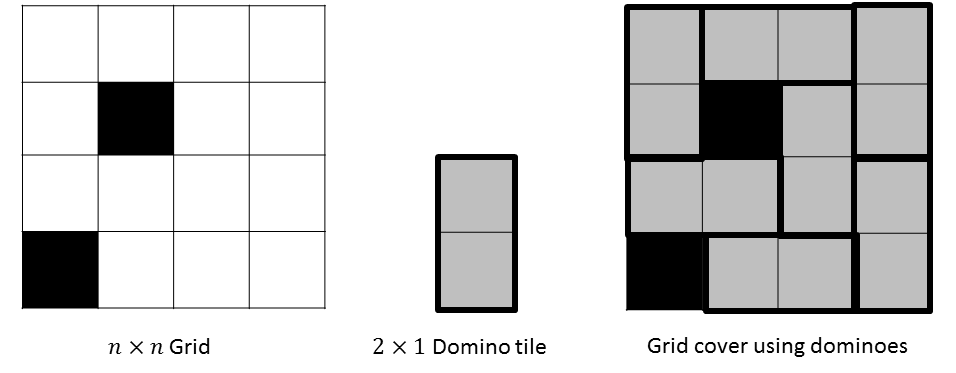
\includegraphics[scale=0.5]{img/domino.png}
\end{center}
Design an algorithm for this problem. Your algorithm should output ``yes" if it is possible to cover the grid and ``no" otherwise. Give running time analysis and proof of correctness.

[Note that you will receive full points if your algorithm has polynomial running time. There are no bonus points for this question.]

    \begin{solution}

        We call a placement of dominos a \textit{tiling} if the conditions mentioned in the problem are satisfied.

I will reduce this problem to finding a perfect matching in a graph.

Consider the graph $G$ constructed as follows:

Let $S$ be the set of all unfilled cells $(i, j)$ which have $i + j$ odd, and let $T$ be the set of all unfilled cells $(i, j)$ which have $i + j$ even. Add an edge between two adjacent cells iff both are unfilled.

        \textbf{Claim 0:} This graph is bipartite.

        \textit{Proof:} Note that we have an edge if and only if the cells are adjacent and empty. Note that for any adjacent cells, the sum of coordinates are $s, s + 1$ for some integer $s$, and
        hence have opposite parities. Hence one of the endpoints of the edge is in $S$ and the other is in $T$. Hence we have shown that for each edge, one endpoint is in $S$ and the other in
        $T$, so no edge has both endpoints in exactly one of the sets $S$ and $T$, showing that the graph is bipartite.

        \textbf{Claim 1:} There is a perfect matching in this graph $\implies$ there is a tiling.

        \textit{Proof:} Suppose a perfect matching exists. Consider a perfect matching. For each edge $(u, v)$ in the graph, since $(u, v)$ is an edge in $G$, $u$ and $v$ must be adjacent cells of the grid which are both unfilled. Hence, we can place a domino covering these two tiles. Now to show that this tiling is valid, note that if there were two dominos intersecting at a cell, then in the perfect matching, we must have had two edges sharing an endpoint, which is impossible due to it being a valid matching. To show that it covers all the unfilled cells, note that since the perfect matching matches all the vertices of the bipartite graph (i.e., for each vertex, there is an edge whose endpoint it is), for each unfilled cell, we must have a domino covering it. Hence we have shown that for a perfect matching in the graph, there is a tiling.

        \textbf{Claim 2:} There is a tiling $\implies$ there is a perfect matching in this graph.

        \textit{Proof:} For any domino, note that it covers two adjacent squares. Either they have consecutive $i$'s and the same $j$ or consecutive $j$'s and the same $i$. In either case, one of the
        cells is in $S$ and the other one is in $T$. Add the edge between these two cells into a set $X$ (and do this for all dominos). Note that since no two dominos overlap, no two edges share a
        vertex, and thus these edges form a matching. Also note that since all cells in $S$ and $T$ are covered by the dominos by the definition of a tiling, this set $X$ of edges is a perfect matching, as required.

Hence we have shown that our problem is equivalent to finding a perfect matching in the bipartite graph $G$. However, we have done this problem in the class, and I will use the routine
        $\textsc{IsThereAPerfectMatching}(G)$ for the algorithm (the details will be summarized in the runtime analysis, nevertheless).

        \textbf{Algorithm:}

        $S$ will be represented implicitly as a list of size equal to the number of unfilled cells at odd sum of coordinates, consisting of elements from $1$ to $|S|$, each representing a cell.
        
        $T$ will be represented implicitly as a list of size equal to the number of unfilled cells at even sum of coordinates, consisting of elements from $|S| + 1$ to $|S| + |T|$, each representing a
        cell.
        
        \begin{algorithmic}
            \Function{IsThereATiling}{$a[1..n, 1..n]$}
                \State let $b[1..n, 1..n]$ := array filled with $-1$ initially \Comment{$b[i, j]$ shall store the vertex number for each cell (i, j) that is unfilled, and -1 if it is filled.}
                \State let $currentIndex := 1$
                \State let $size_S := 0$
                \For{each unfilled cell $(i, j) \in G$}
                    \If{$i + j$ is odd}
                        \State $b[i, j] := currentIndex$
                        \State $currentIndex++$
                    \EndIf
                \EndFor
                \State $size_S := currentIndex - 1$
                \For{each unfilled cell $(i, j) \in G$}
                    \If{$i + j$ is even}
                        \State $b[i, j] := currentIndex$
                        \State $currentIndex++$
                    \EndIf
                \EndFor
                \State $totalVertices := currentIndex - 1$ \Comment{$size_T = totalVertices - size_S$}
                \State let $G$ := graph with vertices $1..totalVertices$
                \For{$i \in \{1\ldots n\}$}
                    \For{$j \in \{1\ldots n\}$}
                        \If{$a[i, j] \neq 0$}
                            \State continue
                        \EndIf
                        \For{$(i', j') \in \{(i + 1, j), (i - 1, j), (i, j + 1), (i, j - 1)\}$}
                            \If{$1 \le i' \le n \land 1 \le j' \le n \land a[i', j'] = 0$}
                                \State add edge between $b[i, j]$ and $b[i', j']$ in $G$
                            \EndIf
                        \EndFor
                    \EndFor
                \EndFor
                \If{\Call{IsThereAPerfectMatching}{$G, \{1 \ldots size_S\}, \{size_S + 1 \ldots totalVertices\}$}}
                    \State output "yes"
                \Else
                    \State output "no"
                \EndIf
            \EndFunction
        \end{algorithmic}

        \textbf{Runtime Analysis:}
        Creation of $b$ takes $O(n^2)$ time. The next two loops take $O(n^2)$ time. Then while constructing the graph, in the innermost loop, we do $O(1)$ work (checks and adding to the end of
        adjacency lists etc), and hence we do $O(n^2)$ work in creating the graph.

        Internally the perfect matching routine finds a bipartite matching and checks if the sizes of the two parts are the same and equal to the size of the max matching of the graph. This is done by
        the Ford Fulkerson algorithm after creating a network with the same vertices and two additional vertices for the source and the sink. Since the size of the max matching equals the max flow in the built network,
        and since the size of the max matching is at most $n^2$, the max flow is at most $n^2$. 

        The number of edges in this graph is at most $O(n^2)$ as well since each vertex in the original graph has degree bounded above by 4,
        and the number of edges in the network is the number of edges in the original graph + size of $S$ + size of $T$ (due to connections between the source and $S$, and $T$ and the sink). The number of vertices in
        the network is at most $n^2 + 2$ as well, and hence in $O(n^2)$. Hence the complexity is $O((V + E)C)$ which is in $O(n^2 \times n^2) = O(n^4)$, and the overall complexity is also $O(n^4)$.


    \end{solution}

\end{questions}
\end{document}

